\documentclass{article}
\usepackage{graphicx}
\usepackage{fancyhdr}
\usepackage{lipsum}
\usepackage{amsmath}

% Configuración de la página
\pagestyle{fancy}
\fancyhf{}
%\fancyhead[L]{} % Eliminamos la imagen del encabezado en las siguientes páginas
%\fancyhead[R]{Autor: Tu Nombre}
%\fancyhead[C]{Título del Documento}
\fancyfoot[C]{\thepage}

\renewcommand{\headrulewidth}{0pt} % Elimina la línea de la cabecera

\begin{document}

% Primera página
\thispagestyle{fancy} % Aplica el estilo solo a esta página
\begin{titlepage}
    \centering
    \vspace*{2cm}
    {
\includegraphics[width=8cm]{imagenes/logo.png}\par} % Ajusta el nombre de la imagen y su tamaño
    \vspace{1cm}
    {\Huge LAB1: Diseño de sistemas digitales\par}
    \vspace{2cm}
    {\Large Jonatan Stiven Restrepo Lora\par}
    \vspace{0.5cm}
    {\Large Otro Nombre\par} % Agrega el nombre del otro autor
    \vspace{0.5cm}
    {\Large Universidad de Antioquia\par} % Agrega el nombre de la universidad
    \vfill
    {\large \today\par}
\end{titlepage}

\section{Introducción}
Se desea crear un circuito que permita hacer la suma de 16 números guardados en un vector, 
siguiendo el siguiente algoritmo:
\[
\sum_{n=0}^{16} (A_n + A_{n+1})
\]
Entre los componentes que se deben utilizar para desarrollar la solución están los Flip-Flops
tipo \textbf{\textit{JK}}

\section{Almacenamiento}

\subsection{Creación del Vector}
Se creó una unidad de almacenamiento el cual pudiera contener un número de 8 bits y a la vez 
permitirá almacenar un número predeterminado, hasta que llegara el nuevo número por el que se reemplazaría.
\begin{figure}[h] % "h" indica que la figura se coloque aquí, aunque LaTeX puede ajustar su posición
    \centering
    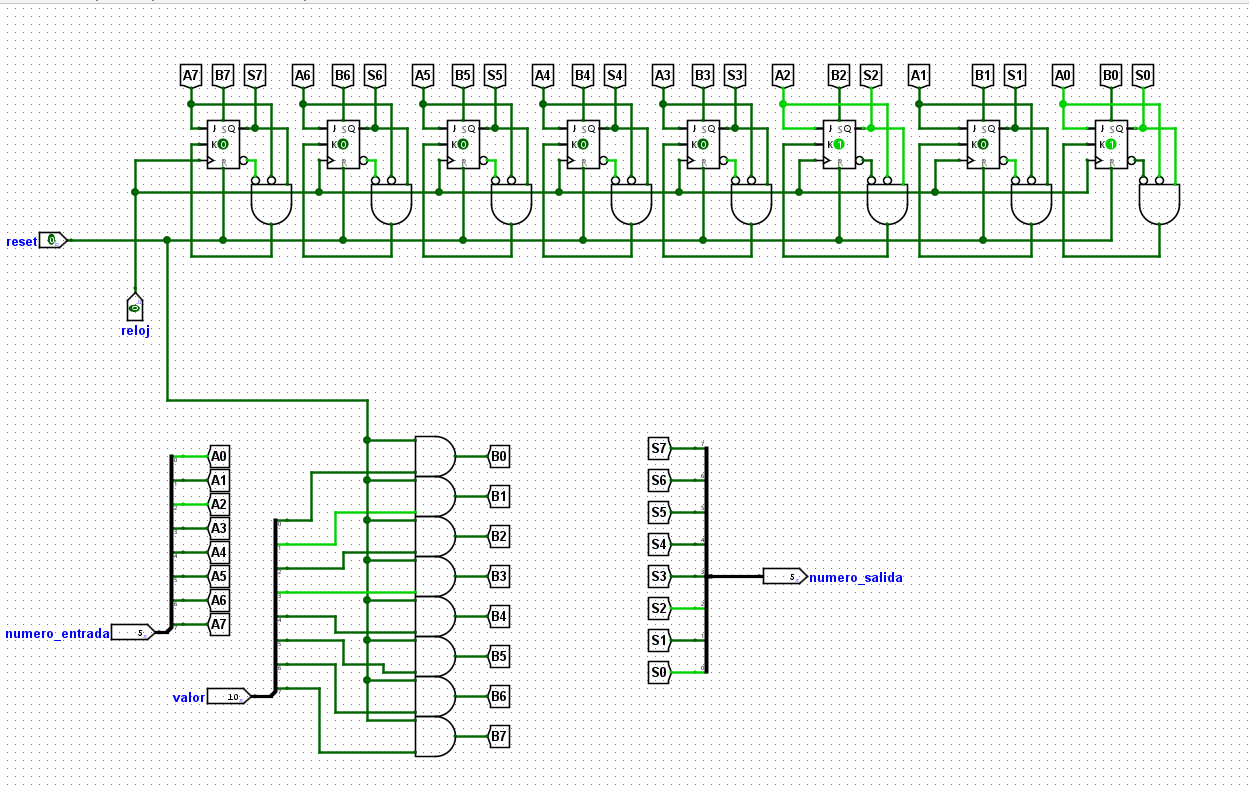
\includegraphics[width=0.8\textwidth]{imagenes/unidad_almacenamiento.png} % Ajusta el nombre de la imagen y el ancho según sea necesario
    \caption{Unidad de almacenamiento} % Agrega la leyenda aquí
    \label{fig:arreglo} % Etiqueta para hacer referencia a la figura en el texto
\end{figure}

Así, de esta manera se podría crear de forma sencilla el vector de 16 posiciones y para el cual se permitiría 
almacenar números predeterminados. Además, se implementó una lógica para que solo escribiera en los arreglos 
correctos según la posición solicitada por el algoritmo y diario se retorne los numeros $A_n$ y $A_{n+1}$

\begin{figure}[h] % "h" indica que la figura se coloque aquí, aunque LaTeX puede ajustar su posición
    \centering
    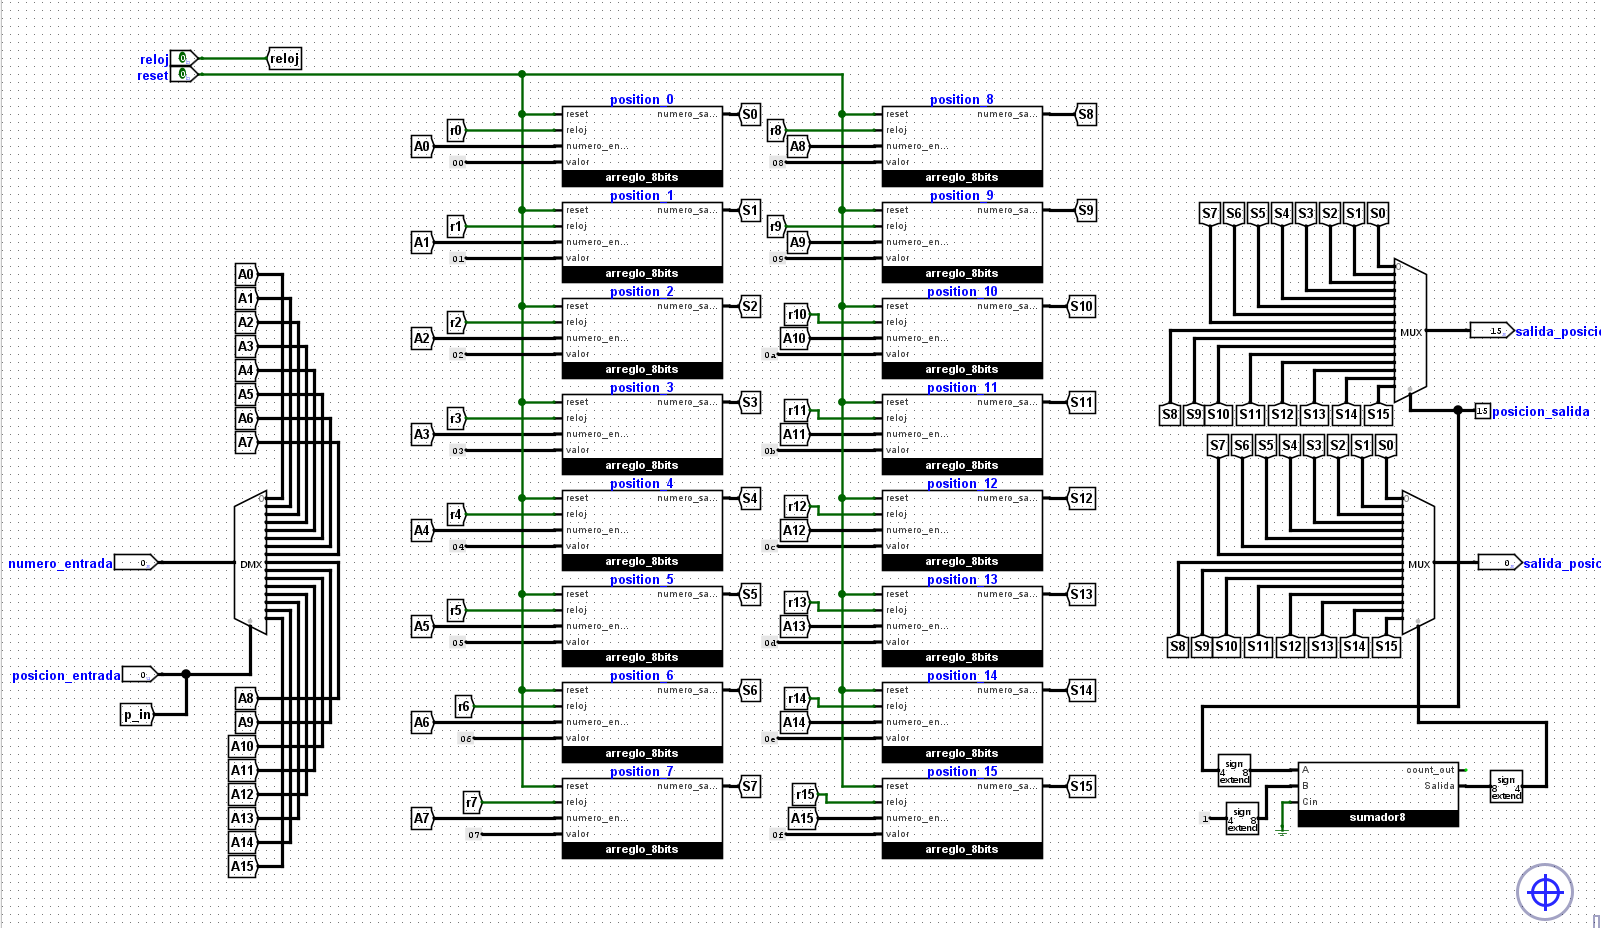
\includegraphics[width=0.8\textwidth]{imagenes/vector.png} % Ajusta el nombre de la imagen y el ancho según sea necesario
    \caption{Vector de 16 posiciones} % Agrega la leyenda aquí
    \label{fig:arreglofull} % Etiqueta para hacer referencia a la figura en el texto
\end{figure}
\newpage
\section{Sumador}
Se construye primero un sumador de un bit full y con base a este se procede a construir uno para 8 bits 
que es la cantidad máxima para este ejercicio.
\begin{figure}[h]
    \centering
    \begin{minipage}{0.45\textwidth} % ajusta el ancho de la primera imagen
      \centering
      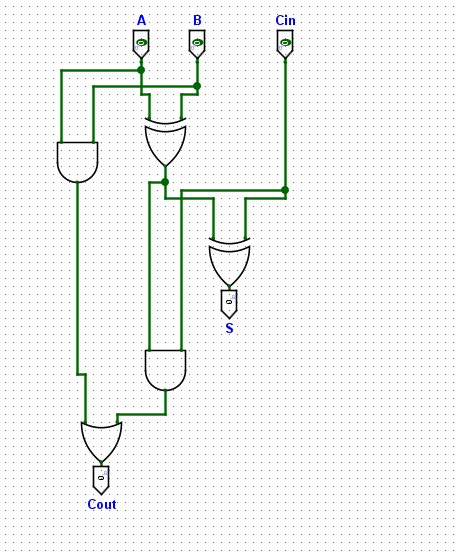
\includegraphics[width=\linewidth]{imagenes/sumador.png} % reemplaza "imagen1" con el nombre de tu primera imagen
      \caption{Sumador completo de 1 bit}
      \label{fig:sumador}
    \end{minipage}
    \hfill
    \begin{minipage}{0.45\textwidth} % ajusta el ancho de la segunda imagen
      \centering
      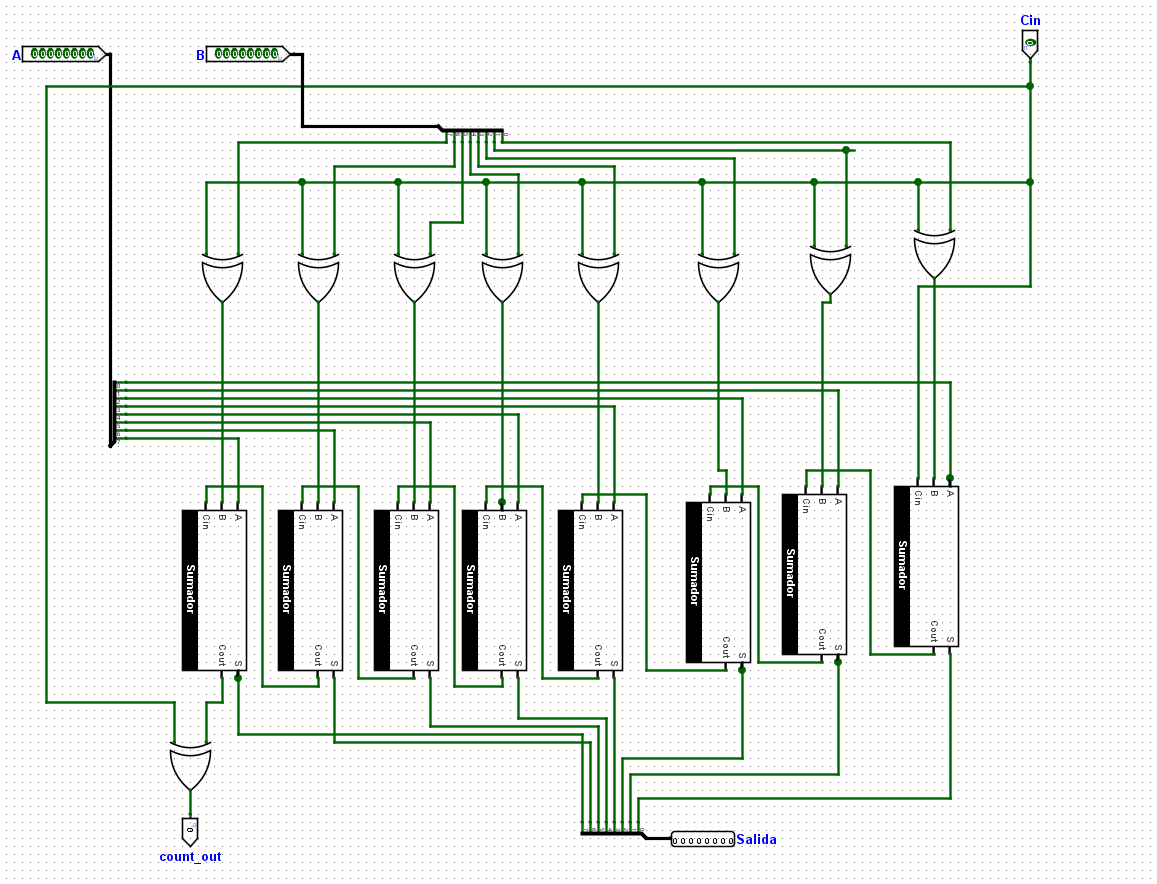
\includegraphics[width=\linewidth]{imagenes/sumador8.png} % reemplaza "imagen2" con el nombre de tu segunda imagen
      \caption{Sumador completo de 8 bits}
      \label{fig:sumador8}
    \end{minipage}
\end{figure}

\section{Contadores}
\subsection{Contador unidad}
Para este ejercicio se creó un contador de 4 bits (16 posiciones posibles) con el flip-flop tipo Jk 
conectados en cascada, el cual ayudaría para saber qué posición del vector guardar los datos, en que 
fase del algoritmo se encuentra y el estado de la máquina.
\begin{figure}[h] % "h" indica que la figura se coloque aquí, aunque LaTeX puede ajustar su posición
    \centering
    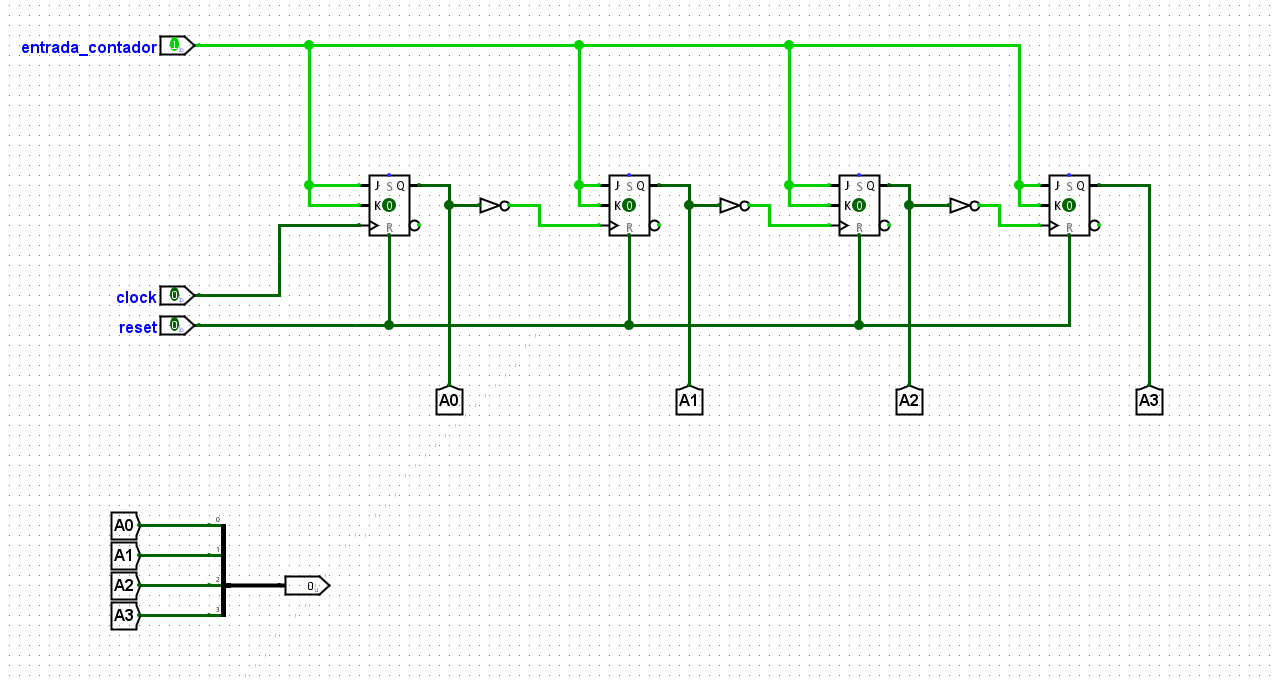
\includegraphics[width=0.8\textwidth]{imagenes/contador.png} % Ajusta el nombre de la imagen y el ancho según sea necesario
    \caption{Contador de 4 bits} % Agrega la leyenda aquí
    \label{fig:contador} % Etiqueta para hacer referencia a la figura en el texto
\end{figure}

\subsection{Contador par}
Se creó un contador par, el cual da las posiciones $\eta = \{ 0, 2, 4, 6, 8, 10, 12, 14 \}$, esto con el 
fin de seguir con la lógica implementada en el vector donde se retorna los números en las posiciones 
$A_n$ \& $A_{n+1}$.
\begin{figure}[h] % "h" indica que la figura se coloque aquí, aunque LaTeX puede ajustar su posición
    \centering
    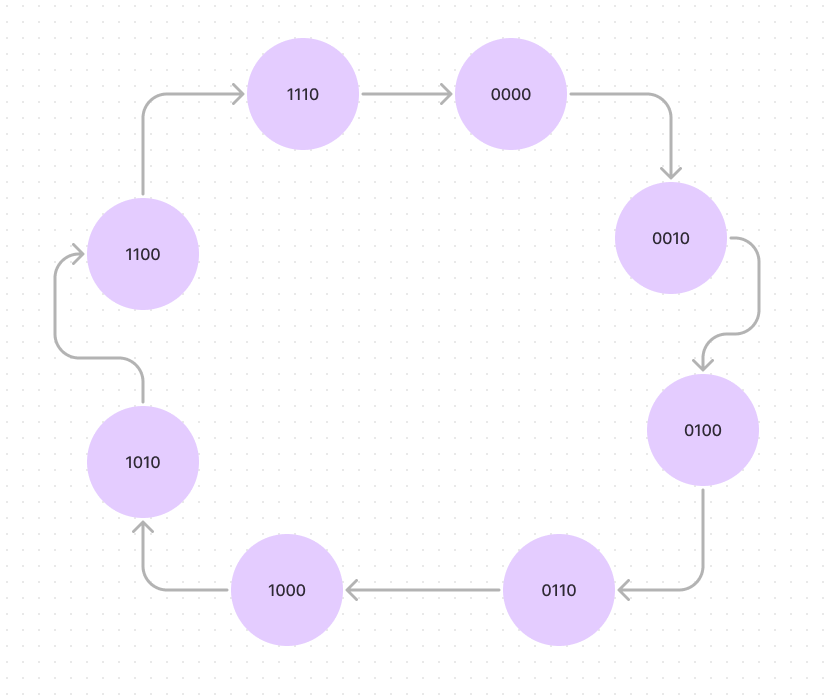
\includegraphics[width=0.5\textwidth]{imagenes/contador_par_diagrama.png} % Ajusta el nombre de la imagen y el ancho según sea necesario
    \caption{Diagrama contador par} % Agrega la leyenda aquí
    \label{fig:diagramacontadorpar} % Etiqueta para hacer referencia a la figura en el texto
\end{figure}
\newpage

Para llevar a cabo la implementación de dicho contador sé continuo con la creación de la tabla extendida 
y la simplificación con los mapas K.
\begin{figure}[h]
    \centering
    \begin{minipage}{0.45\textwidth} % ajusta el ancho de la primera imagen
      \centering
      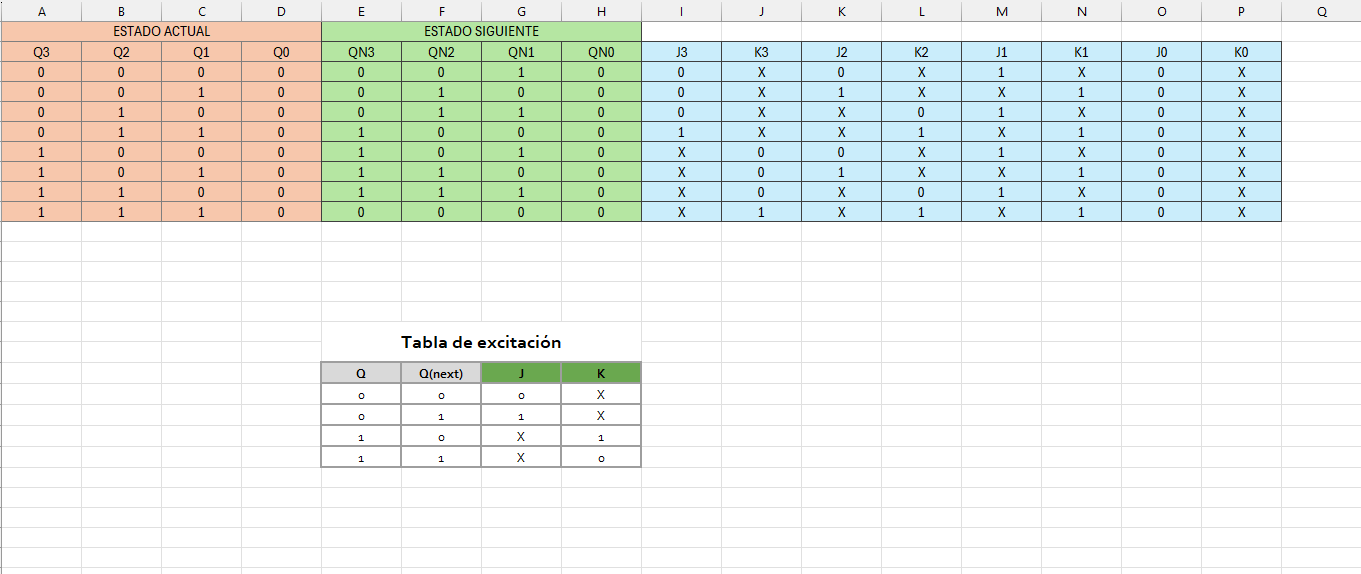
\includegraphics[width=\linewidth]{imagenes/CONTADOR_PAR_TABLA.png} % reemplaza "imagen1" con el nombre de tu primera imagen
      \caption{Tabla extendida contador par}
      \label{fig:tablacontadorpar}
    \end{minipage}
    \hfill
    \begin{minipage}{0.45\textwidth} % ajusta el ancho de la segunda imagen
      \centering
      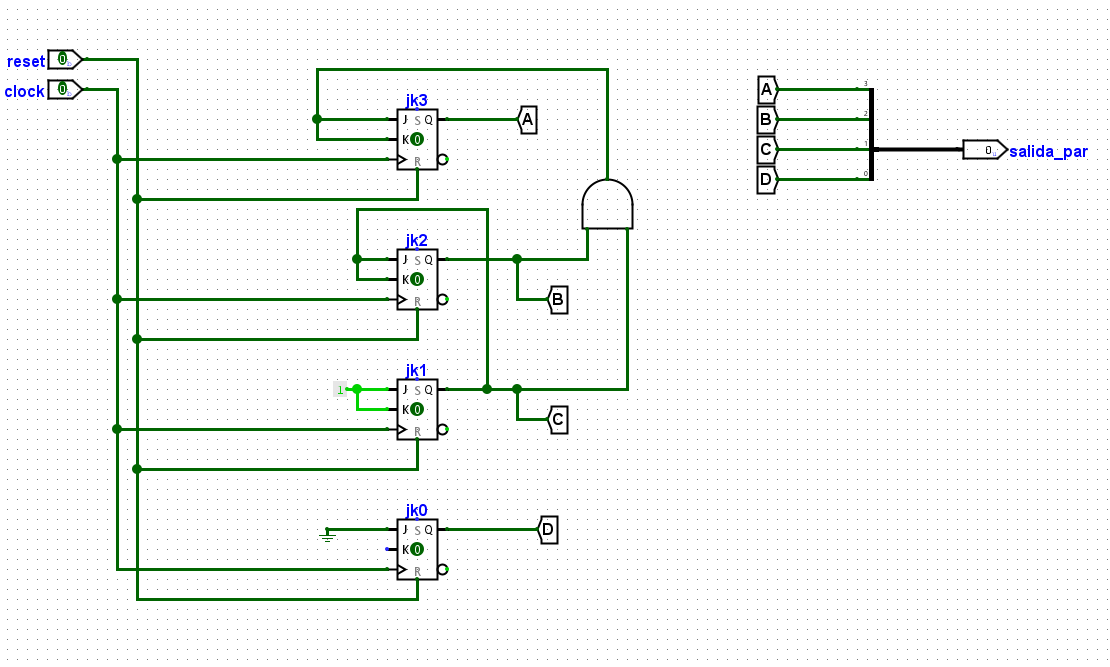
\includegraphics[width=\linewidth]{imagenes/contador_par_circuito.png} % reemplaza "imagen2" con el nombre de tu segunda imagen
      \caption{Circuito contador par}
      \label{fig:circuitocontadorpar}
    \end{minipage}
\end{figure}

\begin{figure}[h]
    \centering
    \begin{minipage}{0.45\textwidth} % ajusta el ancho de la primera imagen
      \centering
      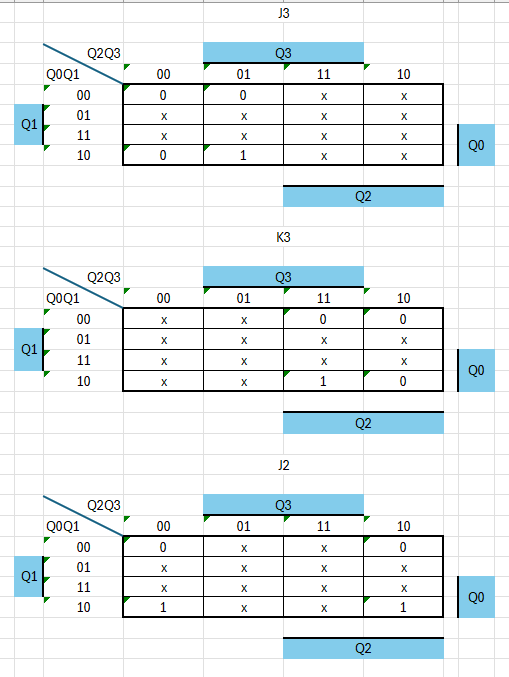
\includegraphics[width=\linewidth]{imagenes/mapask_contador_par_1.png} % reemplaza "imagen1" con el nombre de tu primera imagen
      \caption{Mapas K contador par}
      \label{fig:mapaskcontadorpar}
    \end{minipage}
    \hfill
    \begin{minipage}{0.45\textwidth} % ajusta el ancho de la segunda imagen
      \centering
      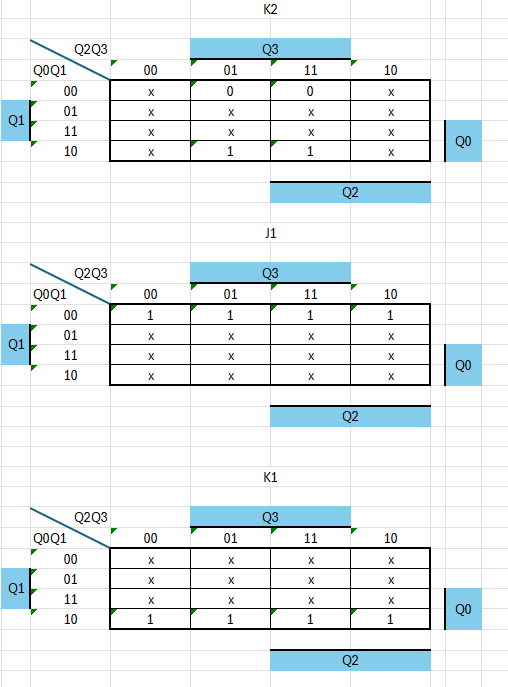
\includegraphics[width=\linewidth]{imagenes/mapask_contador_par_2.png} % reemplaza "imagen2" con el nombre de tu segunda imagen
      \caption{Mapas K contador par}
      \label{fig:mapaskcontadorpar}
    \end{minipage}
\end{figure}
\newpage

\begin{figure}[h] % "h" indica que la figura se coloque aquí, aunque LaTeX puede ajustar su posición
    \centering
    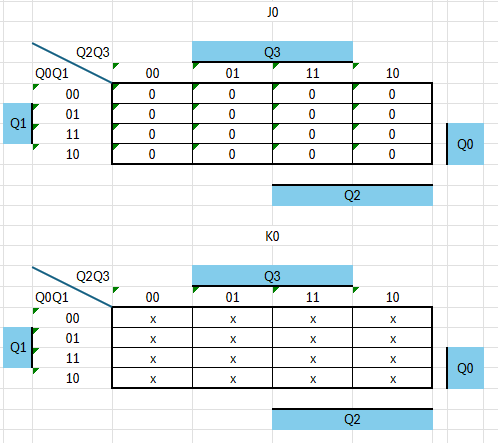
\includegraphics[width=0.5\textwidth]{imagenes/mapask_contador_par_3.png} % Ajusta el nombre de la imagen y el ancho según sea necesario
    \caption{mapas k contador par} % Agrega la leyenda aquí
    \label{fig:mapaskcontadorpar} % Etiqueta para hacer referencia a la figura en el texto
\end{figure}
Las expresiones simplificadas son las siguientes:
\begin{itemize}
    \item $J3 = Q2 \cdot Q1$
    \item $K3 = Q2 \cdot Q1$
    \item $J2 = Q1$
    \item $K2 = Q1$
    \item $J1 = 1$
    \item $K1 = 1$
    \item $J0 = 0$
    \item $K0 = X$
\end{itemize}

\section{Visualizador}
Para poder cumplir con las especificaciones de poder ver los números $A_n$ \& $A_{n+1}$ en cada ciclo 
del algoritmo, la suma correspondiente al mismo ciclo, la face del algoritmo y el estado actual de la máquina, 
fue necesario crear los siguientes componentes:

\subsection{Decodificador 7 segmentos}
Se creó un decodificador de 7 segmentos el cual recibe 4 bits y representa los valores de 0 al 9.
\begin{figure}[h] % "h" indica que la figura se coloque aquí, aunque LaTeX puede ajustar su posición
    \centering
    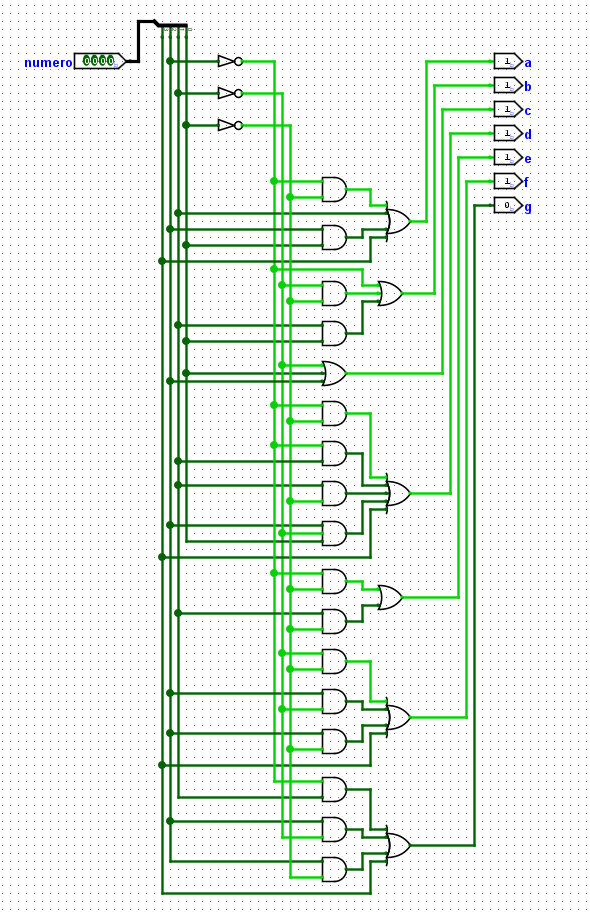
\includegraphics[width=0.5\textwidth]{imagenes/circuito_deco.png} % Ajusta el nombre de la imagen y el ancho según sea necesario
    \caption{Circuito Decodificador 7 segmentos} % Agrega la leyenda aquí
    \label{fig:deco7seg} % Etiqueta para hacer referencia a la figura en el texto
\end{figure}
\newpage

\subsection{Complemento a 2}
Se construyo un circuito que hiciera el complemento a 2, para una entrada de 8 bits. Dicho complemento 
funciona solo para números negativos.
\begin{figure}[h] % "h" indica que la figura se coloque aquí, aunque LaTeX puede ajustar su posición
    \centering
    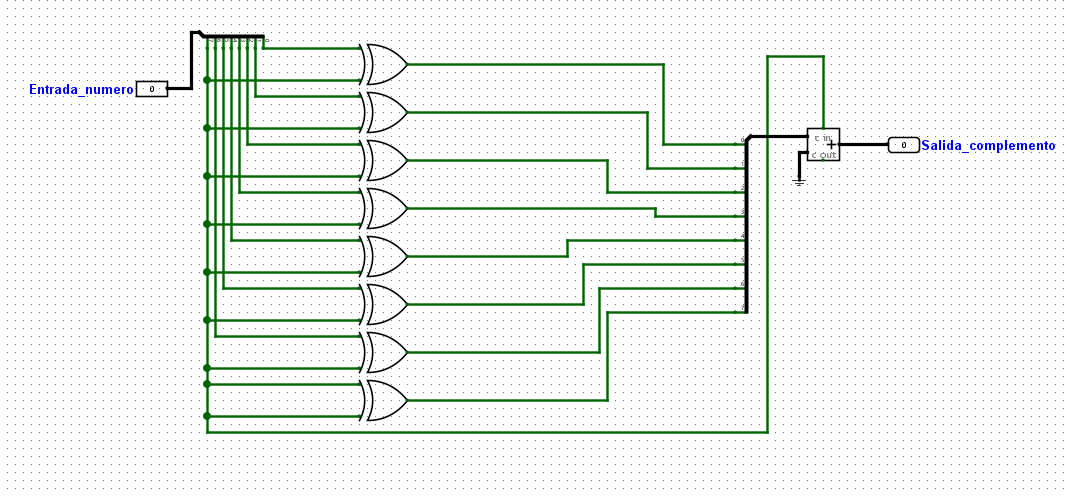
\includegraphics[width=0.5\textwidth]{imagenes/complemento_2.png} % Ajusta el nombre de la imagen y el ancho según sea necesario
    \caption{Circuito Complemento a dos} % Agrega la leyenda aquí
    \label{fig:complemento} % Etiqueta para hacer referencia a la figura en el texto
\end{figure}

\subsection{Construcción Visualizador}
Los componentes anteriores fueron necesarios para poder crear un componente que me permitiera obtener 
las unidades, decenas y centenas de un número, así como también su signo:
\newpage
\begin{figure}[h]
    \centering
    \begin{minipage}{0.45\textwidth} % ajusta el ancho de la primera imagen
      \centering
      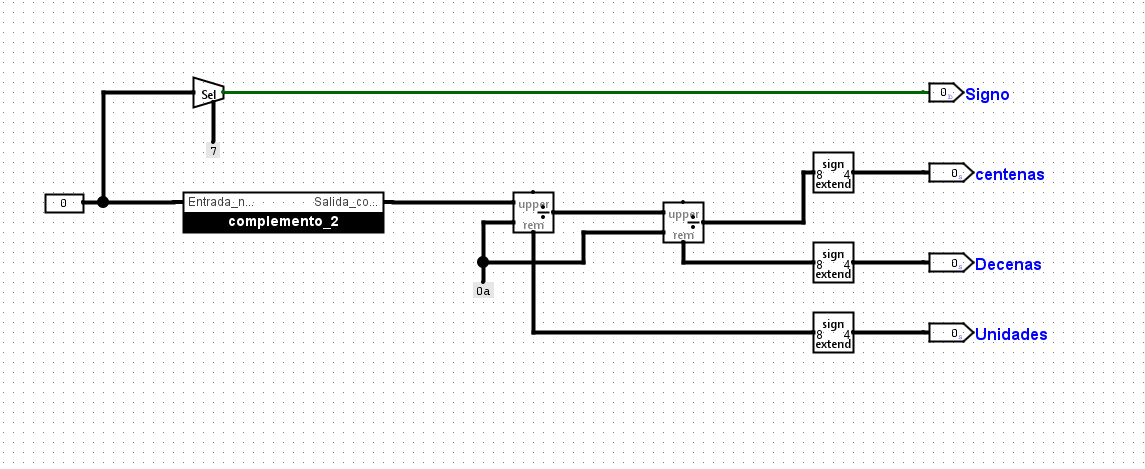
\includegraphics[width=\linewidth]{imagenes/view_number.png} % reemplaza "imagen1" con el nombre de tu primera imagen
      \caption{Circuito desglosé número}
      \label{fig:viewnumber}
    \end{minipage}
    \hfill
    \begin{minipage}{0.45\textwidth} % ajusta el ancho de la segunda imagen
      \centering
      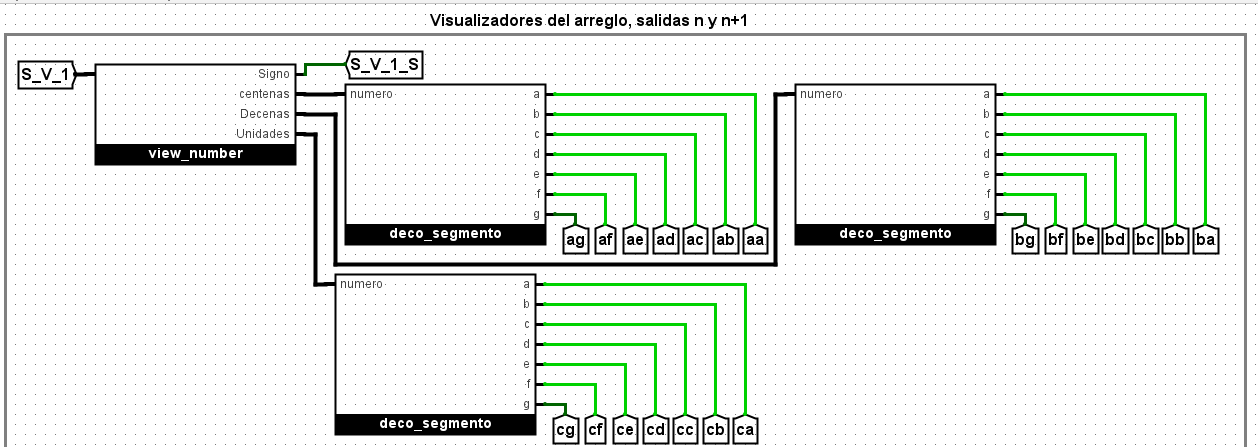
\includegraphics[width=\linewidth]{imagenes/view_number_selector.png} % reemplaza "imagen2" con el nombre de tu segunda imagen
      \caption{Circuito unificado}
      \label{fig:viewnumberunificado}
    \end{minipage}
\end{figure}
\begin{figure}[h] % "h" indica que la figura se coloque aquí, aunque LaTeX puede ajustar su posición
    \centering
    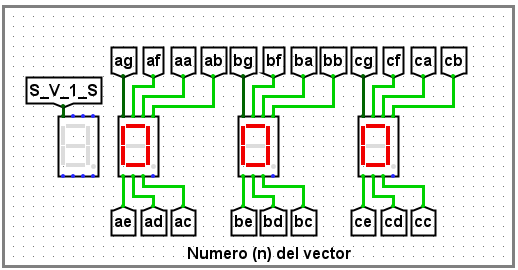
\includegraphics[width=0.5\textwidth]{imagenes/view_number_full.png} % Ajusta el nombre de la imagen y el ancho según sea necesario
    \caption{Resultado Visualizador} % Agrega la leyenda aquí
    \label{fig:visualizadorfull} % Etiqueta para hacer referencia a la figura en el texto
\end{figure}

\section{Máquina de estados}
Para poder llevar a cabo el algoritmo de reducción, se construyo una máquina de estados, dependiendo de la 
entrada de 2 bits que, representa la fase en la que se encuentra, realiza cierta cantidad de ciclos y cuando 
termine genera una salida de \textbf{1}, para de esta forma poder controlar el reset de los contadores y otros 
componentes:
\begin{figure}[h] % "h" indica que la figura se coloque aquí, aunque LaTeX puede ajustar su posición
    \centering
    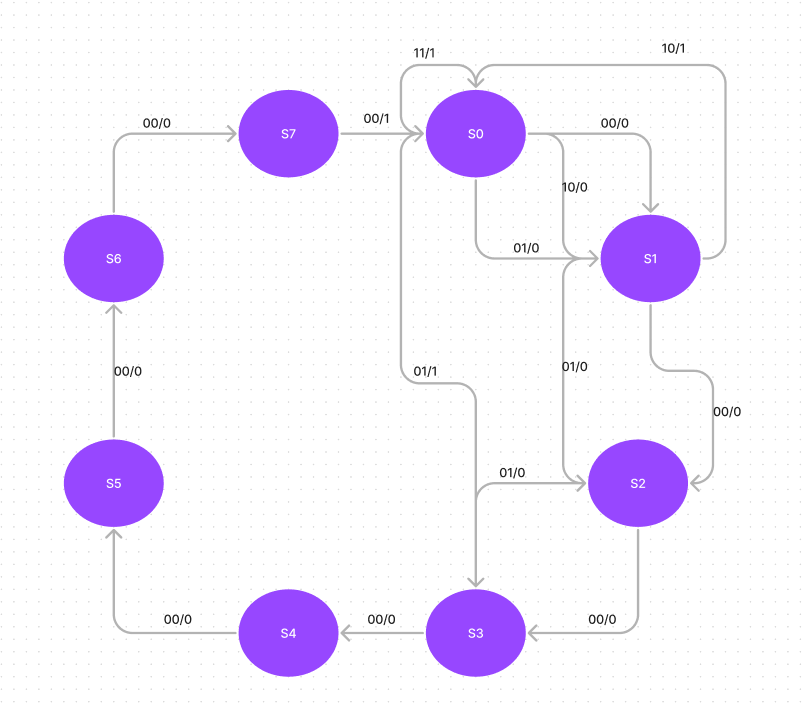
\includegraphics[width=0.5\textwidth]{imagenes/diagrama_maquina_estados.png} % Ajusta el nombre de la imagen y el ancho según sea necesario
    \caption{Diagrama máquina de estados} % Agrega la leyenda aquí
    \label{fig:diagramaestados} % Etiqueta para hacer referencia a la figura en el texto
\end{figure}
\newpage

Como el algoritmo para la suma es de complejidad algorítmica $O(\log_2(n))$, significa que para las 16 
posiciones del vector, solo usaremos como máximo 8 estados para la primera iteración, 4 para la segunda, 
2 para la tercera, 1 para la última fase, teniendo en cuanta lo anterior, se evidencia solo 8 estados 
en la máquina.
\begin{figure}[h] % "h" indica que la figura se coloque aquí, aunque LaTeX puede ajustar su posición
    \centering
    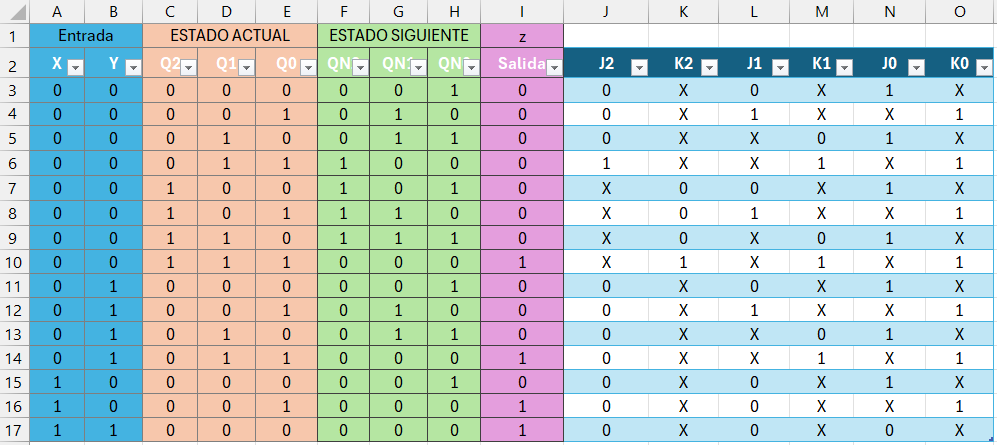
\includegraphics[width=0.5\textwidth]{imagenes/TABLA.png} % Ajusta el nombre de la imagen y el ancho según sea necesario
    \caption{Tabla extendida de la maquina de estados} % Agrega la leyenda aquí
    \label{fig:tablaestados} % Etiqueta para hacer referencia a la figura en el texto
\end{figure}
\begin{figure}[h] % "h" indica que la figura se coloque aquí, aunque LaTeX puede ajustar su posición
    \centering
    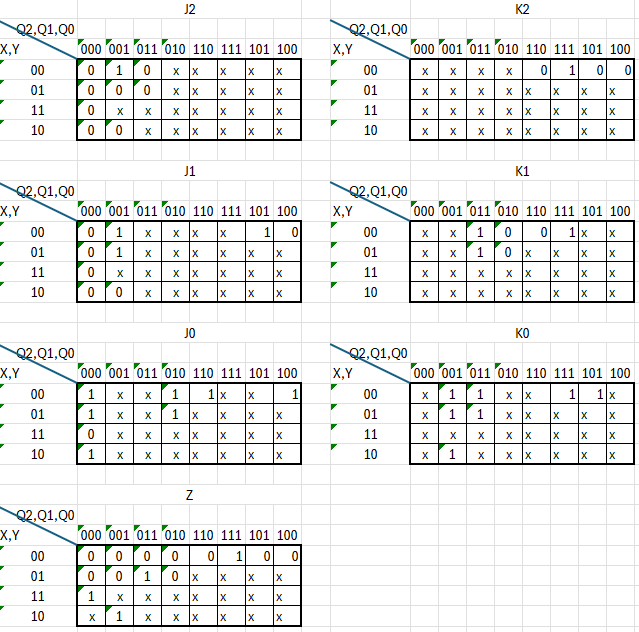
\includegraphics[width=0.8\textwidth]{imagenes/mapask_estados.png} % Ajusta el nombre de la imagen y el ancho según sea necesario
    \caption{Mapas K de la máquina de estados} % Agrega la leyenda aquí
    \label{fig:mapaskestados} % Etiqueta para hacer referencia a la figura en el texto
\end{figure}
\newpage

\textbf{Expresiones minimizadas:}

\begin{align*}
    J0 &= X' + Y' \\
    J1 &= X' + Q0 \\
    J2 &= Y' \cdot Q1 \cdot Q0 \\
    K0 &= 1 \\
    K1 &= Q0 \\
    K2 &= Q1 \cdot Q0 \\
    Z &= Q2 \cdot Q1 \cdot Q0 + Y \cdot Q1 \cdot Q0 + X \cdot Q0 + X \cdot Y
\end{align*}
\begin{figure}[h] % "h" indica que la figura se coloque aquí, aunque LaTeX puede ajustar su posición
    \centering
    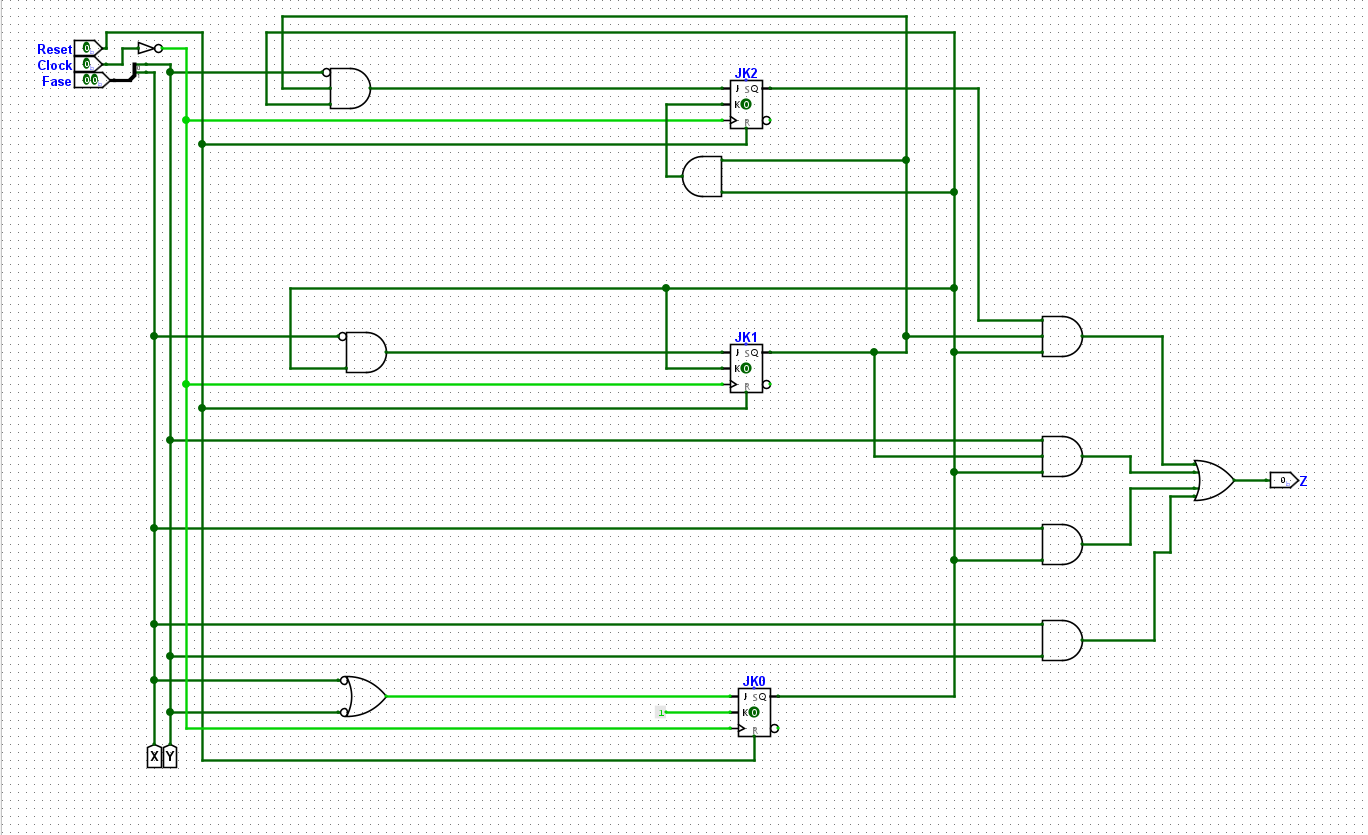
\includegraphics[width=0.8\textwidth]{imagenes/circuito_estados.png} % Ajusta el nombre de la imagen y el ancho según sea necesario
    \caption{Circuito maquina de estados} % Agrega la leyenda aquí
    \label{fig:circuitoestados} % Etiqueta para hacer referencia a la figura en el texto
\end{figure}

\section{Ensamble circuito}
Teniendo en cuenta los componentes antes presentados, se procede a ensamblar cada uno de ellos para poner en 
funcionamiento el algoritmo de suma para un vector de 16 posiciones con 8 bits de entrada.

\subsection{Visualizador}
Con base a los vizualizadores pasados, se construyo uno por cada elemento requerido: 
\textbf{\textit{Número $A_n$ y $A_{n+1}$ del vector, Suma de los números, Fase del algoritmo, Estado actual de la máquina de estados.}}
\newpage
\begin{figure}[h] % "h" indica que la figura se coloque aquí, aunque LaTeX puede ajustar su posición
    \centering
    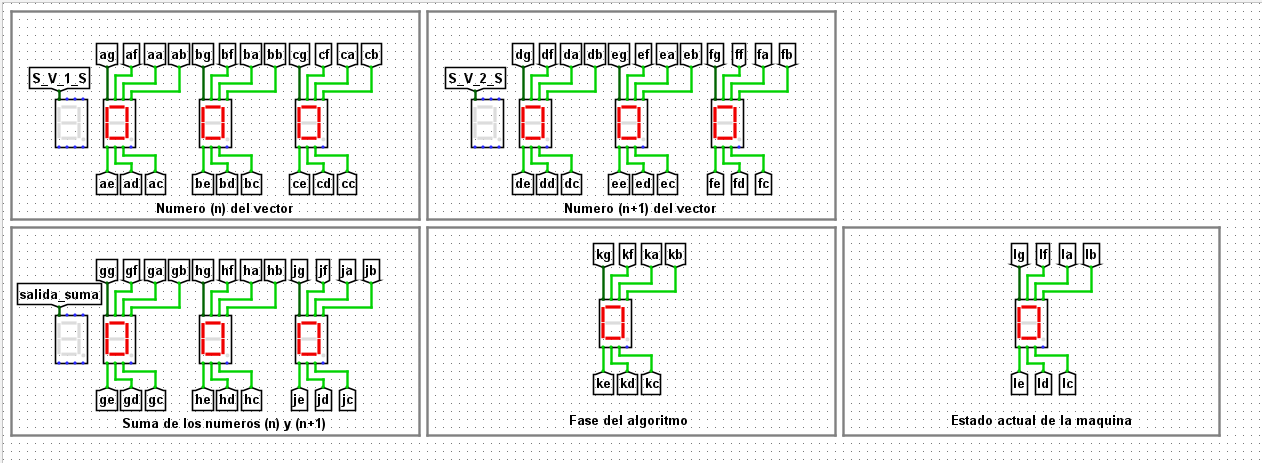
\includegraphics[width=0.8\textwidth]{imagenes/visualizador.png} % Ajusta el nombre de la imagen y el ancho según sea necesario
    \caption{Visualizador de los elementos} % Agrega la leyenda aquí
    \label{fig:Visualizador} % Etiqueta para hacer referencia a la figura en el texto
\end{figure}
\subsection{implementación}
\begin{figure}[h] % "h" indica que la figura se coloque aquí, aunque LaTeX puede ajustar su posición
    \centering
    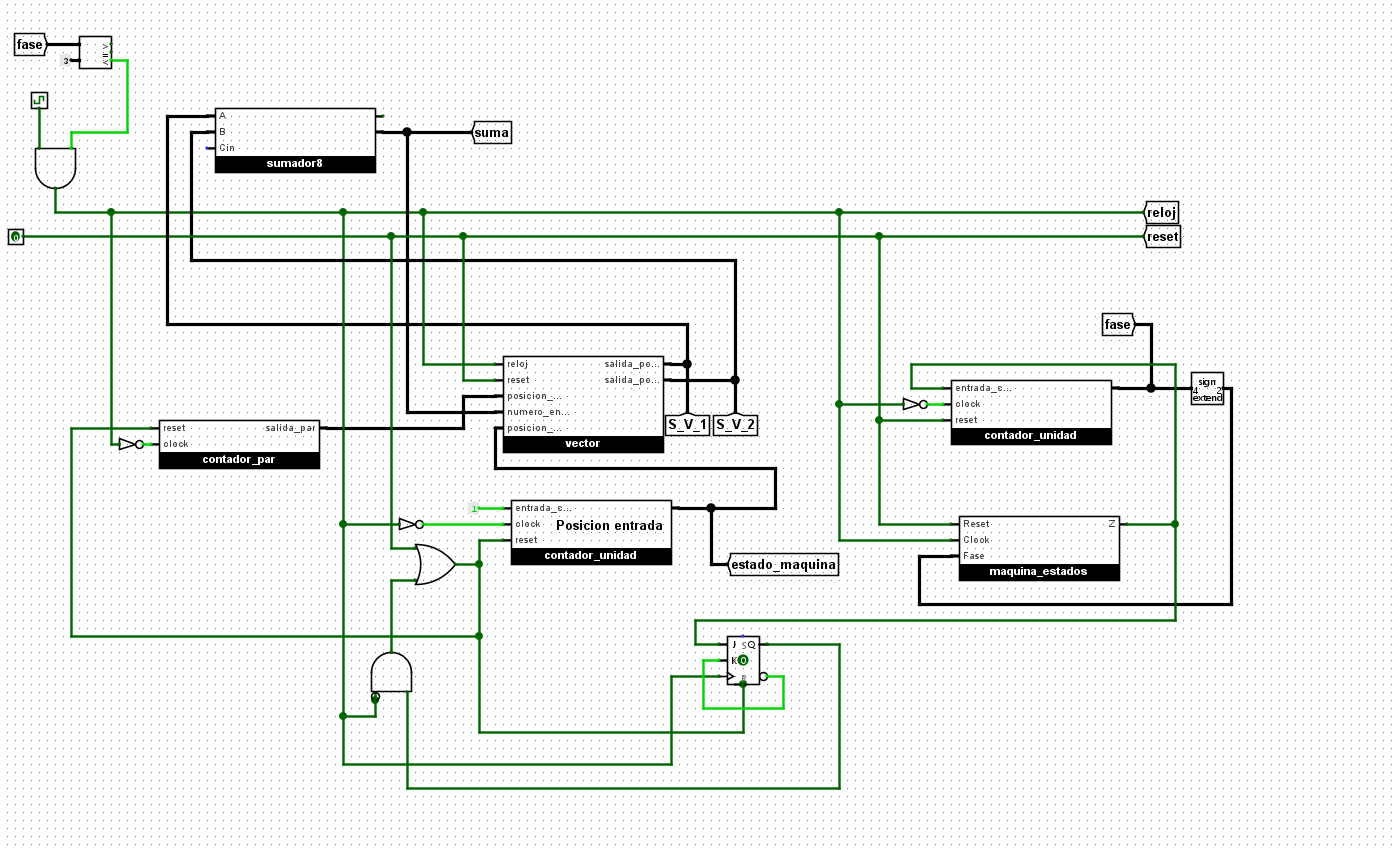
\includegraphics[width=0.8\textwidth]{imagenes/circuito_full.png} % Ajusta el nombre de la imagen y el ancho según sea necesario
    \caption{Implementacion del circuito} % Agrega la leyenda aquí
    \label{fig:circuitofull} % Etiqueta para hacer referencia a la figura en el texto
\end{figure}

Todos los \textbf{contadores} funcionan con flancos de reloj de bajada, para así permitir que el resultado 
de sumar el número $A_n$ \& $A_{n+1}$ se pueda guardar en la posición $\eta$ del vector.
El vector guarda los números con flancos de subida del reloj, de esta manera diario estará guardando los 
datos en la posición correcta.
Con respecto al flip-flop Jk usado, este permite que la última suma correspondiente al estado de la máquina 
se guarda en la posición correcta, dado que por el diseño de la misma cuando está en el último estado activa
la salida que produce un reset en los contadores.
\newpage
\begin{figure}[h] % "h" indica que la figura se coloque aquí, aunque LaTeX puede ajustar su posición
    \centering
    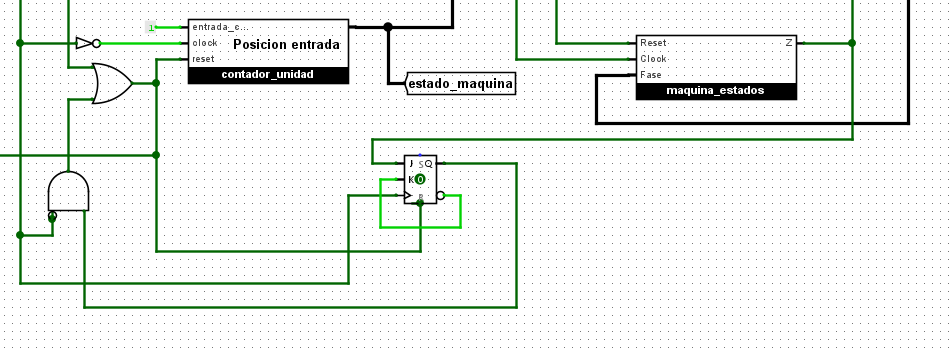
\includegraphics[width=0.8\textwidth]{imagenes/ultimo_ciclo.png} % Ajusta el nombre de la imagen y el ancho según sea necesario
    \caption{Uso del flip-flop para retardar el reset.} % Agrega la leyenda aquí
    \label{fig:ultimociclo} % Etiqueta para hacer referencia a la figura en el texto
\end{figure}

Por último se configuró el circuito para que se detuviera cuando estuviera en la última fase del algoritmo
y así evitar que este corra indefinidamente provocando desbordamiento.
\begin{figure}[h] % "h" indica que la figura se coloque aquí, aunque LaTeX puede ajustar su posición
    \centering
    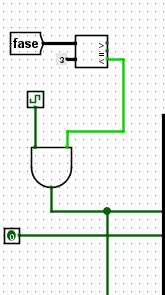
\includegraphics[width=0.3\textwidth]{imagenes/control.png} % Ajusta el nombre de la imagen y el ancho según sea necesario
    \caption{Control fin del algoritmo} % Agrega la leyenda aquí
    \label{fig:control} % Etiqueta para hacer referencia a la figura en el texto
\end{figure}
\end{document}
